\section{Used Hardware}
The following sections will overview the characteristics and the potential of the hardware that has been used in this thesis project. In particular, seven commercially-available boards have been employed: two SensorTile.box devices from ST Microelectronics, two BlueTile boards from the same vendor, and three MetaMotionS from MbientLab. The included sensors, microcontrollers and the available APIs for each one will be listed and explained here. 

\subsection{ST SensorTile.box}
The SensorTile.box from ST Microelectronics (STEVAL-MKSBOX1V1) is a kit that contains all the necessary to start developing IoT applications based on remote motion and environmental data. In particular, the included board presents a set of ST MEMS sensors:
\begin{itemize}
    \item Digital temperature sensor (STTS751)
    \item 6-axis inertial measurement unit (LSM6DSOX)
    \item 3-axis accelerometers (LIS2DW12 and LIS3DHH)
    \item 3-axis magnetometer (LIS2MDL)
    \item Altimeter / pressure sensor (LPS22HH)
    \item Microphone / audio sensor (MP23ABS1)
    \item Humidity sensor (HTS221)
\end{itemize}

      \begin{figure}[ht!]
        \centering
        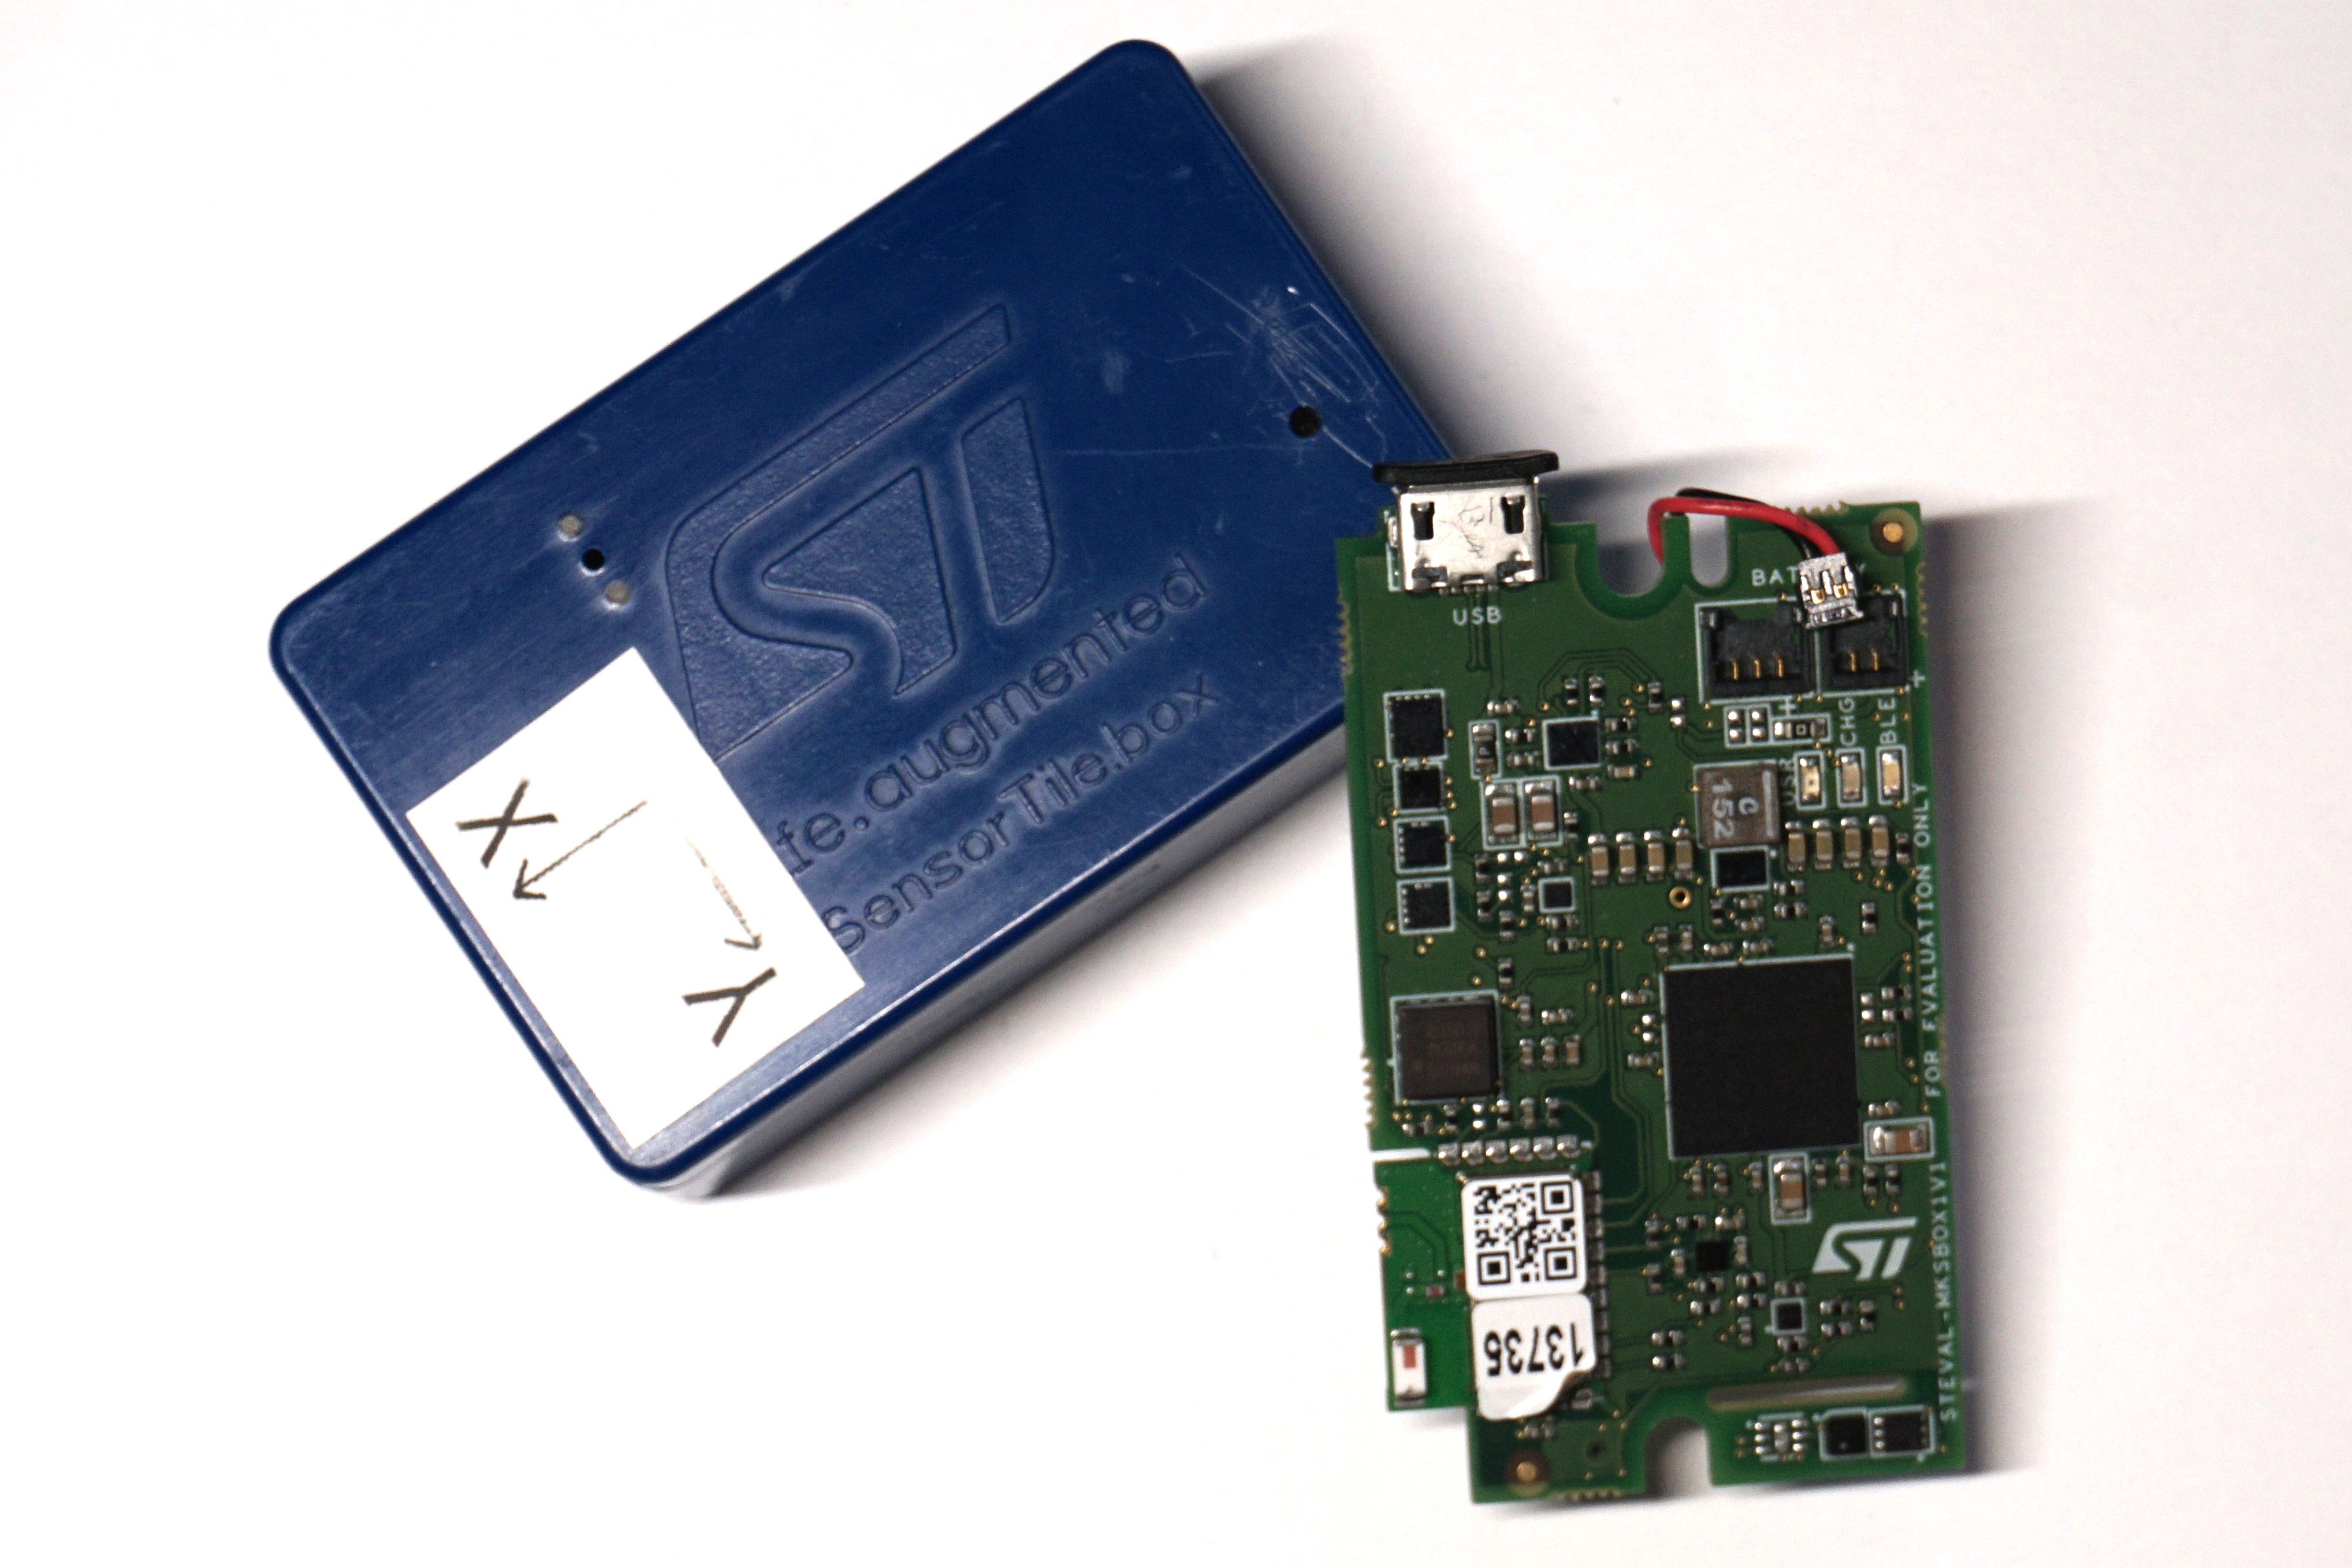
\includegraphics[width=0.75\textwidth]{chap2/figure/stbox.JPG}
        \caption{Image of the SensorTile.box, with the included case.}
        \label{fig:sensortilebox-image}
    \end{figure}

All the data coming from these sensors can be processed with the help of the embedded STM32L4R9 microcontroller, an ARM Cortex-M4 based processor containing DSP and FPU units. All the information can be then transmitted with the ST Bluetooth processor BlueNRG-M2, that supports Bluetooth Low Energy 5.2 specifications. 

The board comes with a preinstalled firmware that allows to read the sensor data via ST applications, or to log data inside an SD cart. The Android application also allows some firmware personalization, adding features like sensor fusion, audio FFT and so on. Anyway, there is no functionality that allows time synchronization of any type. 

If any developer wants to modify the firmware, it is possible to connect the peripheral to the computer and write a firmware using the STM32 development environment \cite{STM32dev}. Then, it is possible to write a firmware from scratch or to start from the available firmware examples (from GitHub or the ST website). The developer can then decide if they wants to keep compatibility with the ST applications or not, as they have total freedom on the board behaviour. 

ST offers an extensive set of Hardware Abstraction Layer (HAL) procedures, that makes it easy to develop firmware for the board and access functionality from both the sensors and the Bluetooth Low Energy stack.

Once the firmware is ready, the microcontroller can be flashed by means of ST solutions (ST-Link) or via an USB cable. The STM32CubeProgrammer \cite{STM32CubeProg} is the ST software that allows the programming. 

To conclude the overview, the kit contains a long-life USB-rechargeable battery and a case that provides water and dust resistance.  

\subsection{ST BlueTile}
The BlueTile from ST Microelectronics (STEVAL-BCN002V1B) is a development board containing a full set of MEMS sensors connected to a BlueNRG-2 SoC, that allows Bluetooth Low Energy connectivity. Here's the list of the embedded sensors:
\begin{itemize}
    \item  BALF-NRG-02D3: ultra-miniature balun and harmonic filter
    \item  LSM6DSO: iNEMO 6DoF inertial module, ultra-low power and high accuracy
    \item  LIS2MDL: magnetic sensor, digital output, 50 Gauss magnetic field dynamic range, ultra-low power, high performance, 3-axis magnetometer
    \item  VL53L1X: long range Time-of-Flight sensor based on ST FlightSense technology
    \item  MP34DT05TR-A: MEMS audio sensor omnidirectional digital microphone, 64~dB SNR, -26~dBFS sensitivity, top-port, 122.5~dBSPL AOP
    \item  LPS22HH: ultra-compact piezo-resistive absolute pressure sensor, 260-1260~hPa, digital output barometer, full-mold dust resistant, holed LGA package (HLGA)
    \item  HTS221: capacitive digital sensor for relative humidity and temperature 
\end{itemize}

      \begin{figure}[ht!]
        \centering
        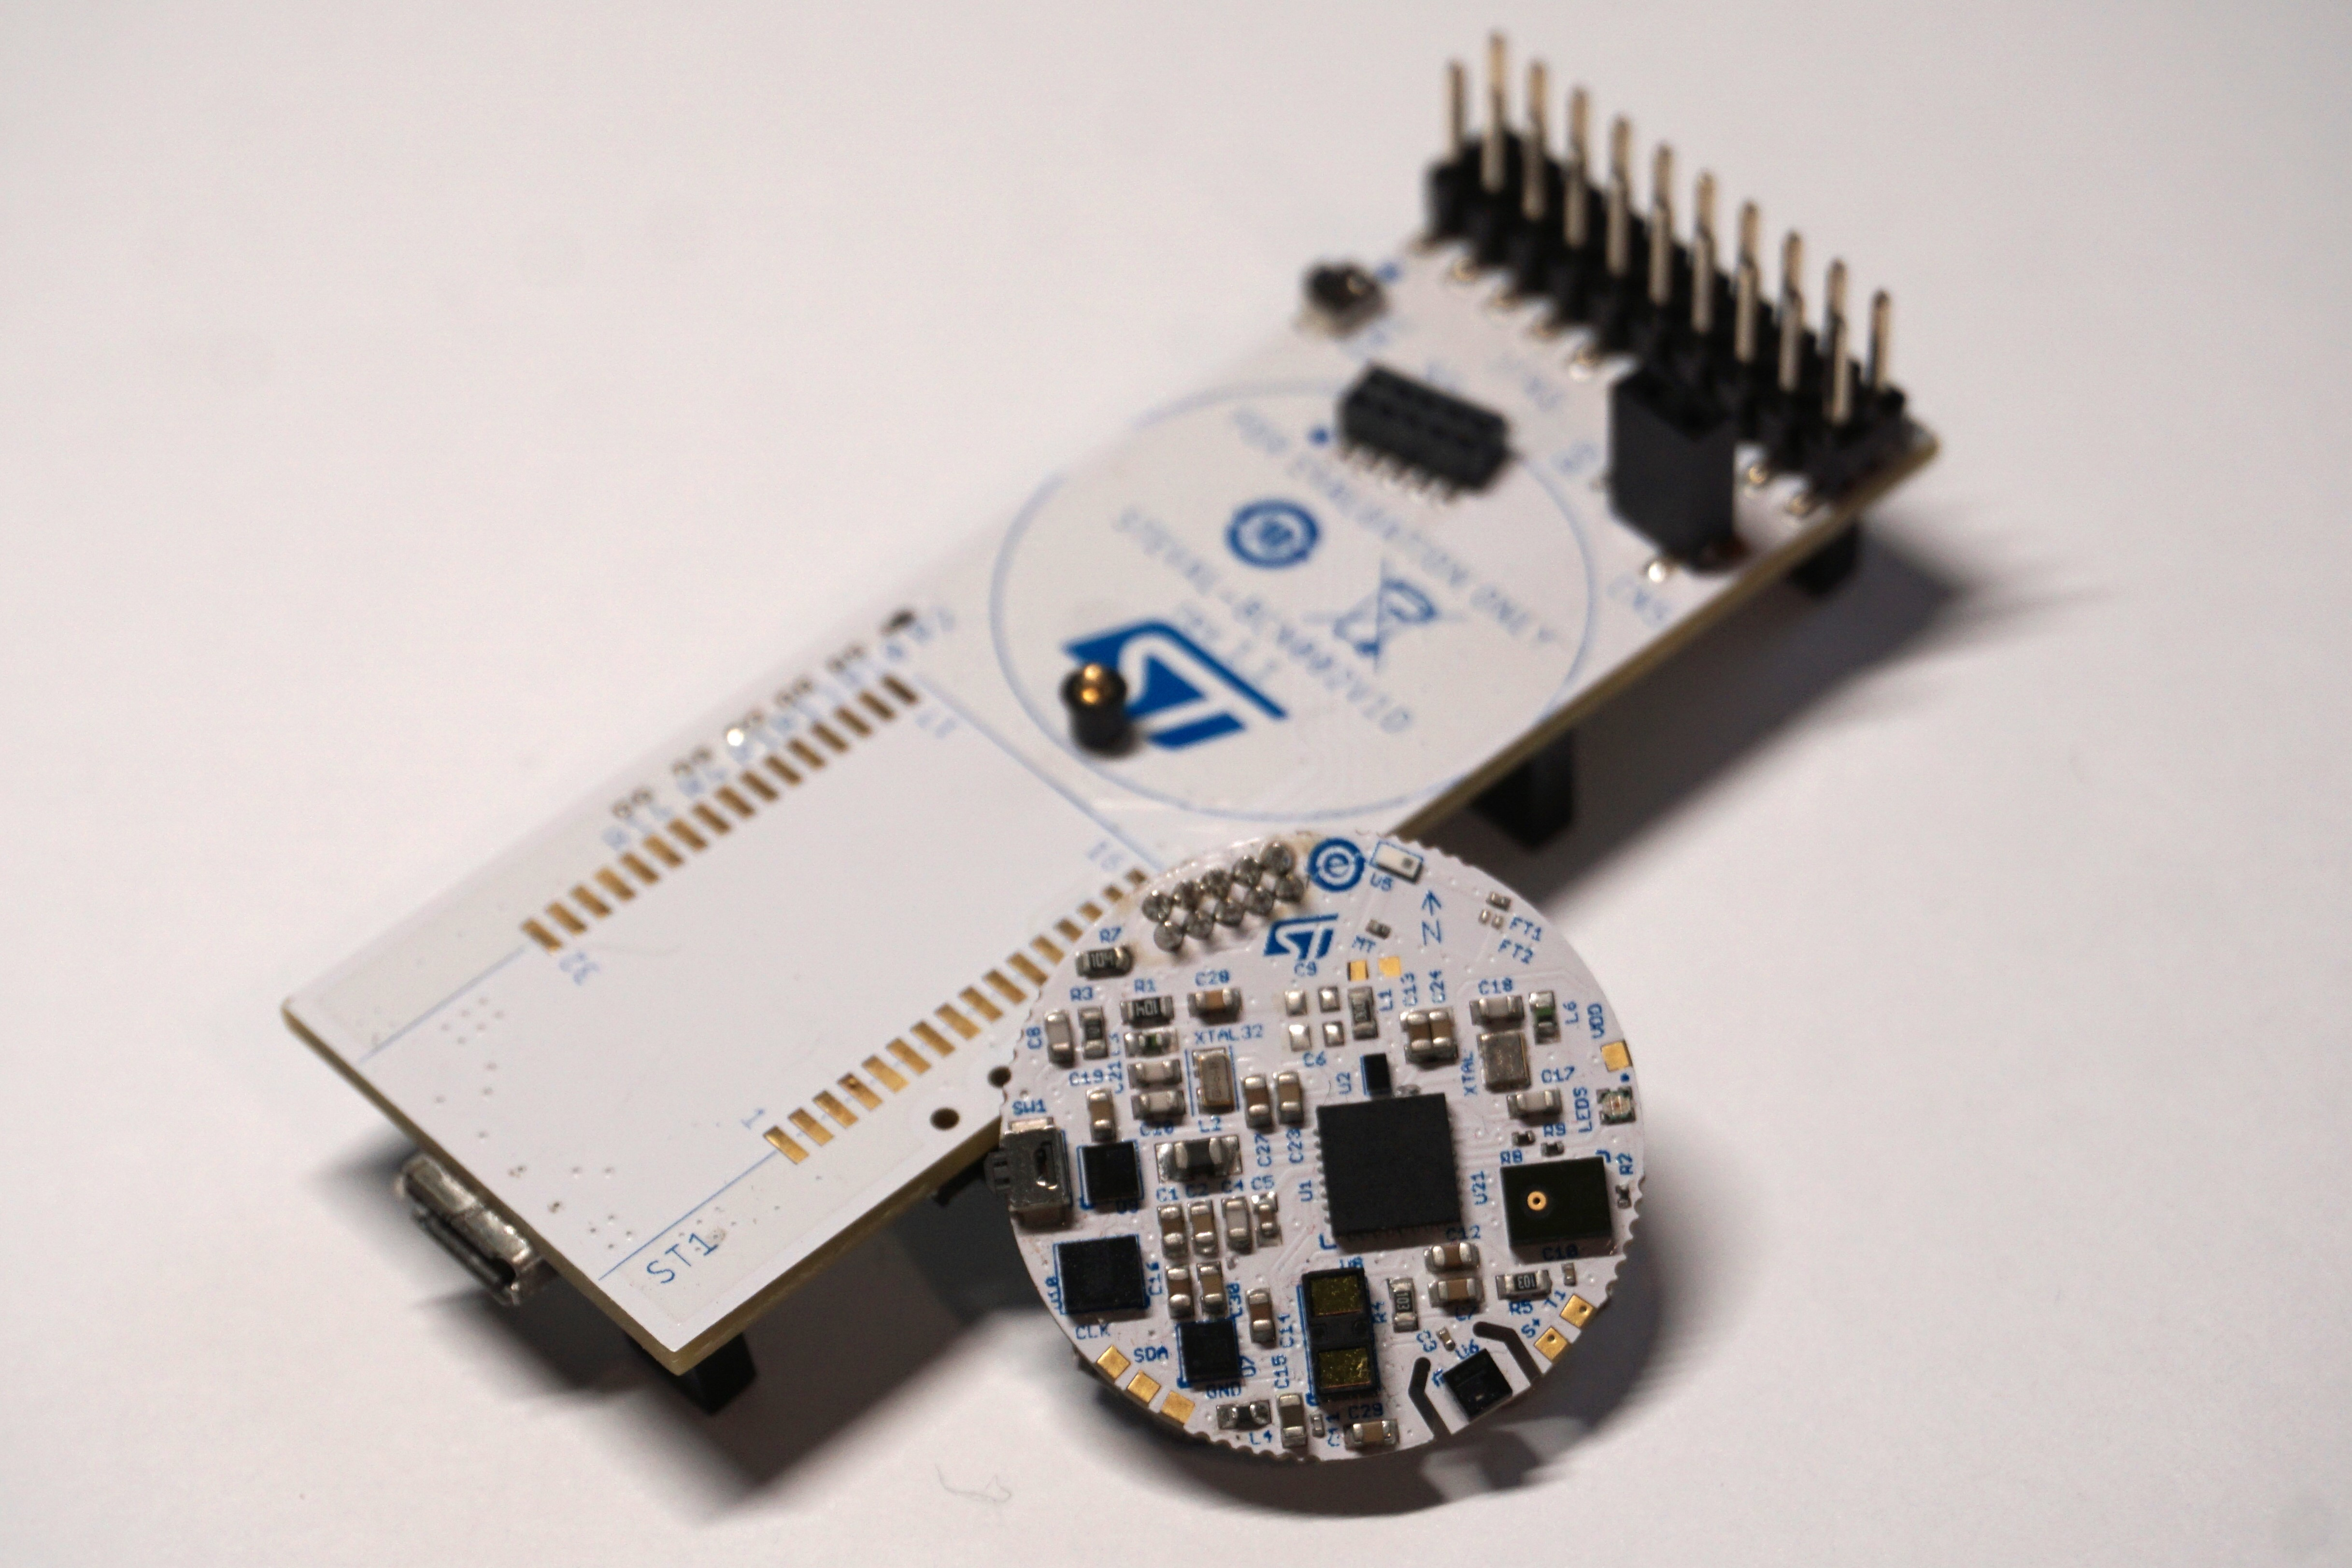
\includegraphics[width=0.75\textwidth]{chap2/figure/btile.JPG}
        \caption{Image of the BlueTile, with its programming board.}
        \label{fig:bluetile-image}
    \end{figure}

To perform elaboration and transmission of the resulting data, the embedded  SoC is a network processor for Bluetooth Low Energy that allows its own Cortex M0 core to be programmed by the user. In this way, no overhead is present, as one chip is enough to perform all the necessary operations for the board. Also in this case, ST released examples and low-level drivers, allowing the board to be programmed at high-level under both the BLE connectivity and sensor configuration aspects. 

The kit also contains a programming board, to which the small BlueTile can be connected: then, it can be programmed by means of a USB cable or a programming interface from ST (ST-link or ST NUCLEO  board), with the ST RF-Flasher software \cite{rfflasher}.

The board can be powered via an USB cable, when connected to its programming board, or via a CR2032 battery. ST advertises the sensors and the microcontroller to be battery-friendly, thanks to some hardware optimizations and their enhanced sleep states.

\subsection{MBIENTLAB MetaMotionS}
While ST solutions give a lot of freedom to the final user, making it easy for them to develop and personalize the firmware of the boards, MBIENTLAB solutions go in a different direction, offering devices with a complete set of sensors that are ready to use. In my case, I had at my disposal three MetaMotionS, containing the following set of sensors:
\begin{itemize}
    \item Bosch BMI270 6-Axis Accelerometer/Gyroscope
    \item Bosch BMM150 3-Axis Magnetometer
    \item Bosch BMP280 Digital Pressure Sensor
    \item Lite-On LTR-329ALS-01 Ambient Light Sensor
    \item I/O analog and digital pins are present for expansion purposes.
\end{itemize}

      \begin{figure}[ht!]
        \centering
        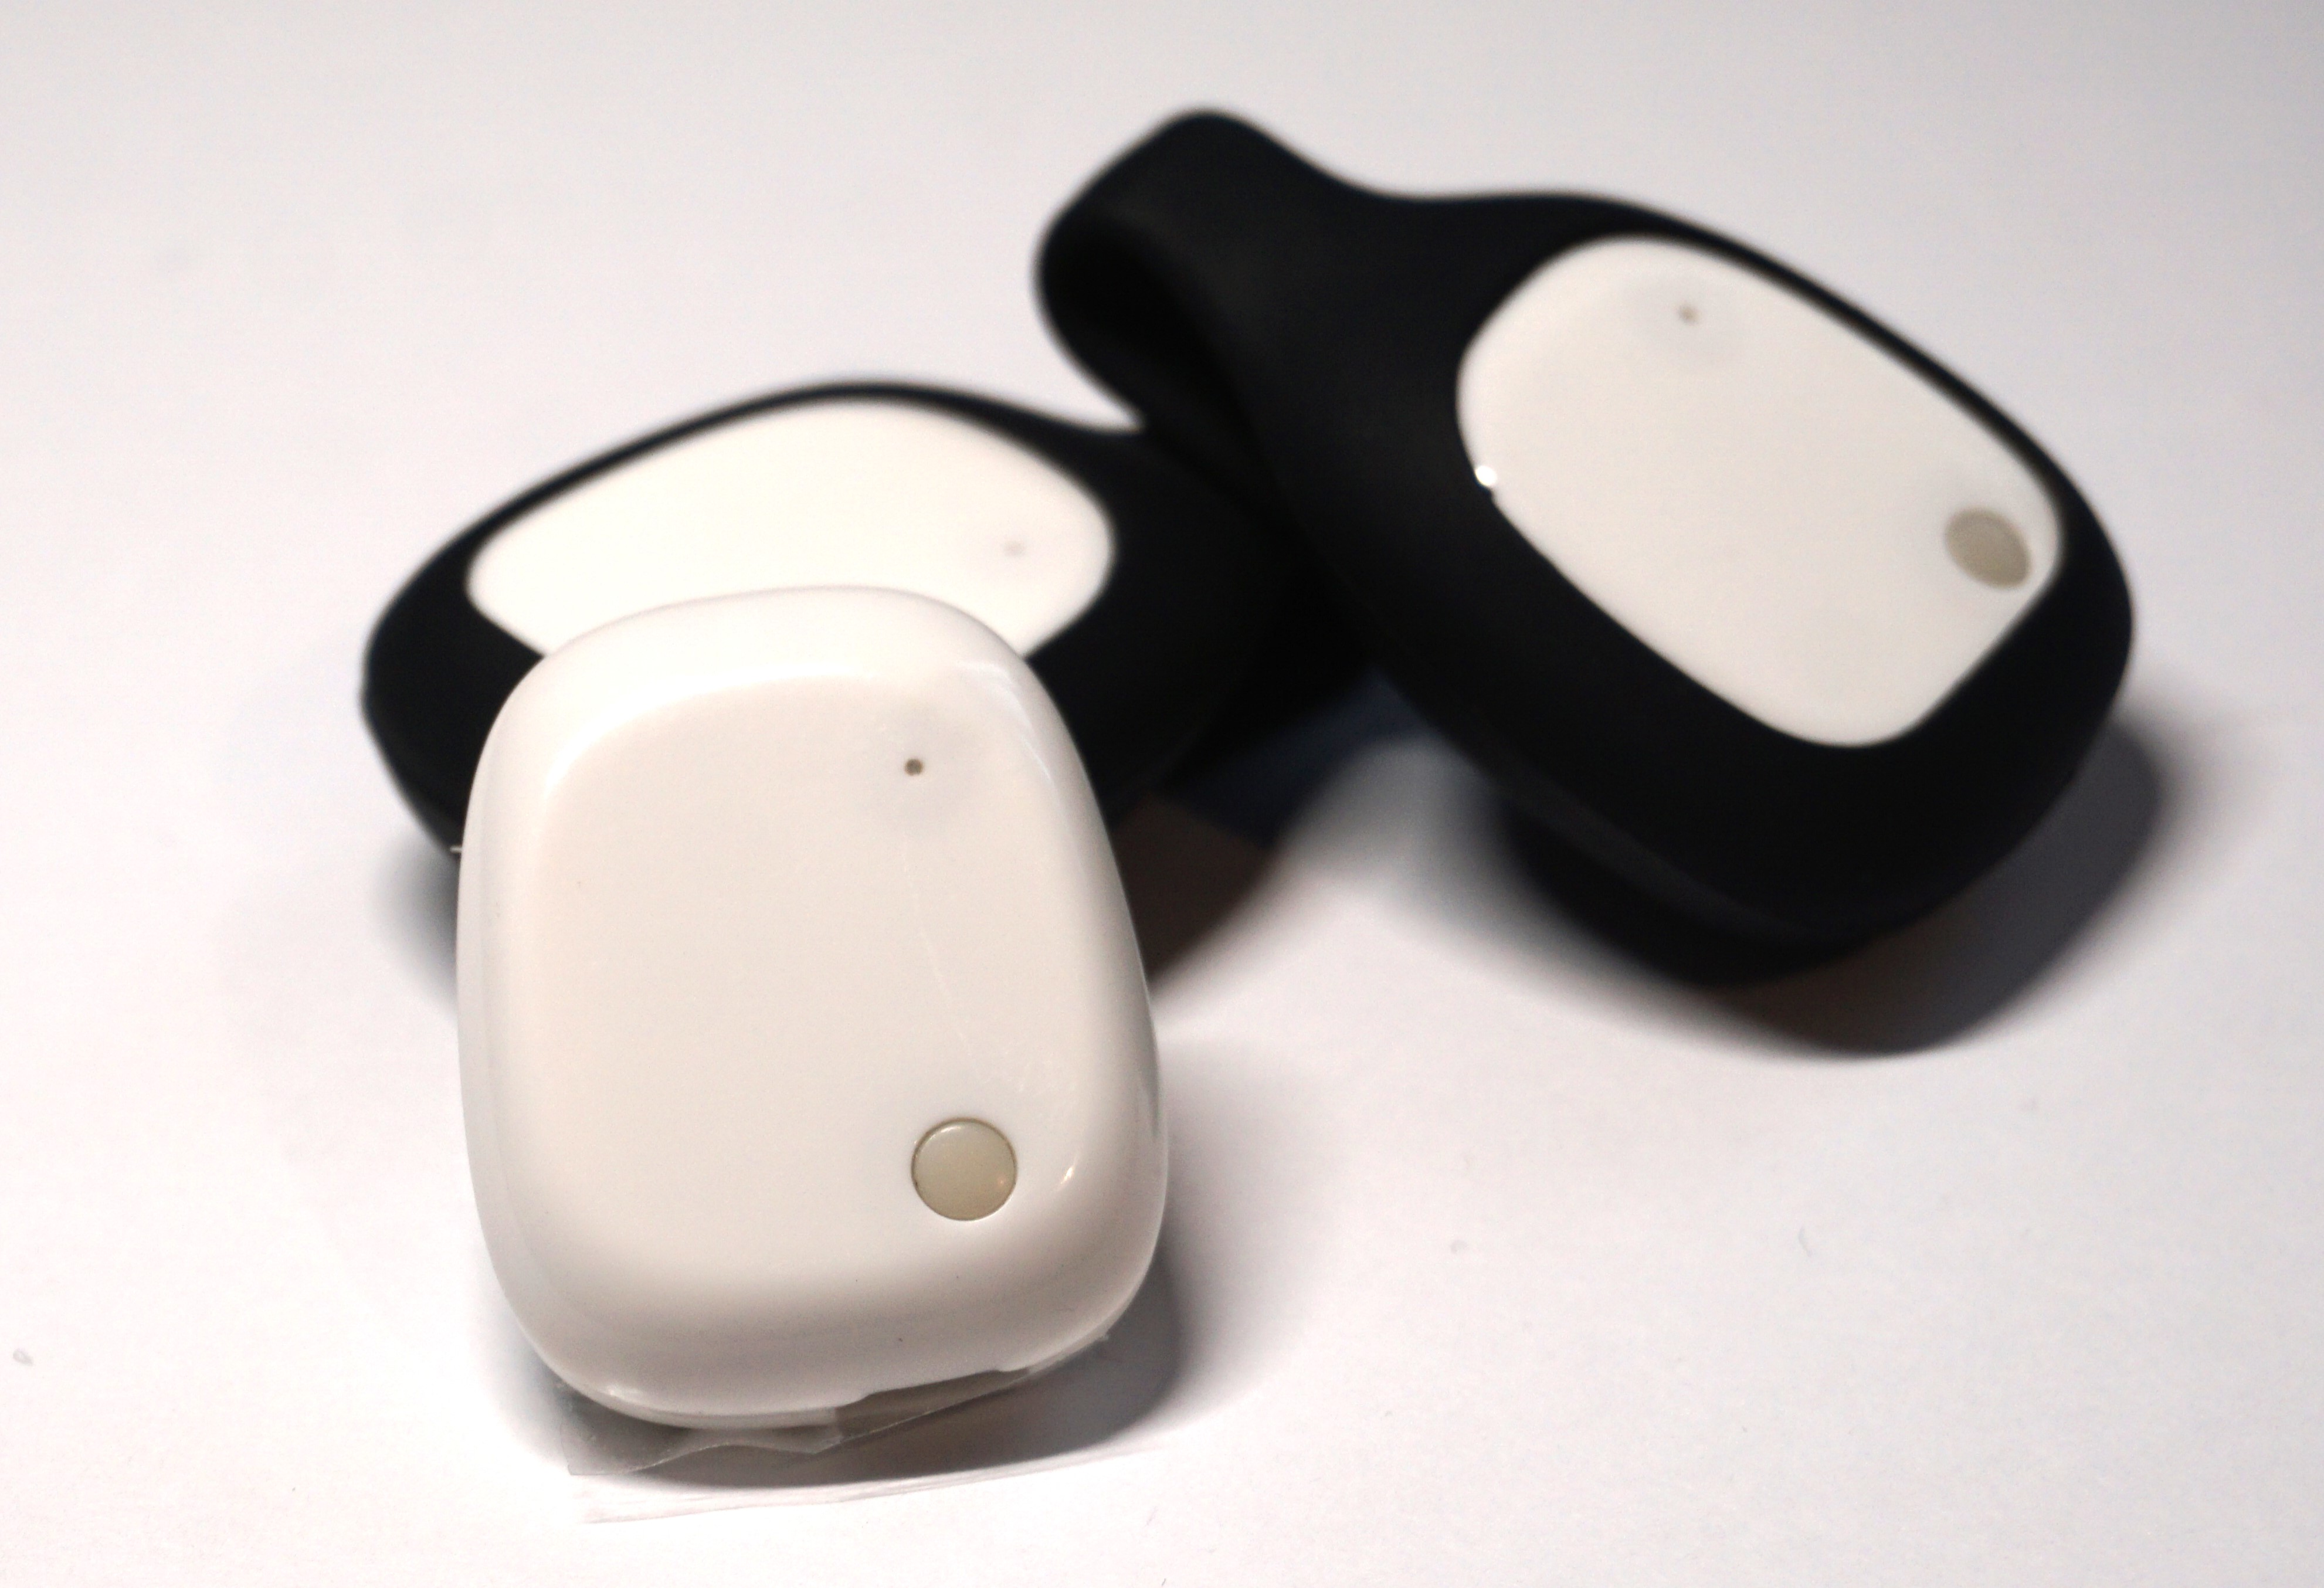
\includegraphics[width=0.75\textwidth]{chap2/figure/mms.JPG}
        \caption{Image of the MetaMotionS devices, with and without the clip accessory.}
        \label{fig:mms-image}
    \end{figure}

All the sensors are connected to a Nordic Semiconductor nRF52840 BLE SoC, which is the network chip whose Cortex-M4 processor allows heavy data elaboration (including 9-axis sensor fusion algorithms). The sensors information can be transmitted via both Bluetooth Low Energy protocols and USB. The provided firmware is closed source and can't be modified. 

The device comes in a water-resistant case enclosure that can be put in (optional) wearable accessories, like clips and wristbands and it contains a USB-rechargeable battery. The mobile application available, MetaBase \cite{metabase}, allows a complete configuration of the sensors, that can be turned on/off and configured in their data rate and precision. Once everything is set-up, the application can start the data recording, that can be streamed directly on the mobile device or saved in the 512~MB internal  memory, to be downloaded later. 

The most interesting part of these products are the open-source APIs that are available \cite{metawearapi}, making the devices easily configurable and usable from any BLE-supported computer or smartpoone with a reduced number of lines of code. In particular, they are available for Android (Java), iOS (Swift), Linux (Javascript, Python), Windows (Python) and already include all the necessary libraries and procedures for Bluetooth connectivity. A C++ library is also available, to be adapted to other operating systems and their Bluetooth stacks. The APIs are well-documented on their website, while their GitHub profile contain a lot of examples ready to be personalized to the user needs. 

To conclude this overview, it is important to add that these boards firmwares already contain a sort of synchronization mechanism. All the data coming from them is precisely timestamped with a UNIX Epoch time, in particular with a millisecond resolution. 
